\chapter{Detailed Design}

etailed design done by specifying algorithm and structure that makes up the interior modules. Usually there are many choice but from the different alternatives available. The one, which offer greatest efficiency, simply functionality is selected based on the relative important of these criteria

\section{Data Dictionary}
A data dictionary provides a complete documentation of all the element of system like data items, data stores(database) and data flow. Data described in data dictionary carries the details of the type, data name, database name, data description and characterization. Data Dictionary covers the whole organization or a database.
Data Dictionary is only collection of the element definition.

\section{Input and output Design}

		Considering all o the interaction of user with the system be in most effective and simplified way.                All the input forms are designed in she user will be able to use them in very eff possibilities needed by the user................
		
		
		% This section type your project contents 
		
		
		
\subsection{Admin}

\begin{center}
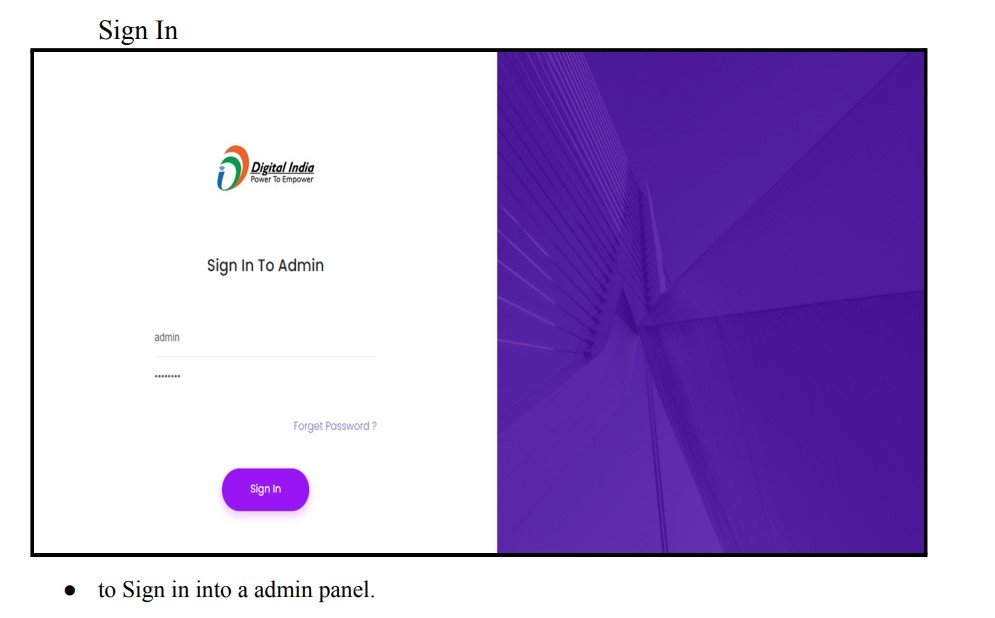
\includegraphics[height=9cm,width=14cm]{Admin/Sign.jpg}
\end{center}


% This section type your project contents 

\begin{center}
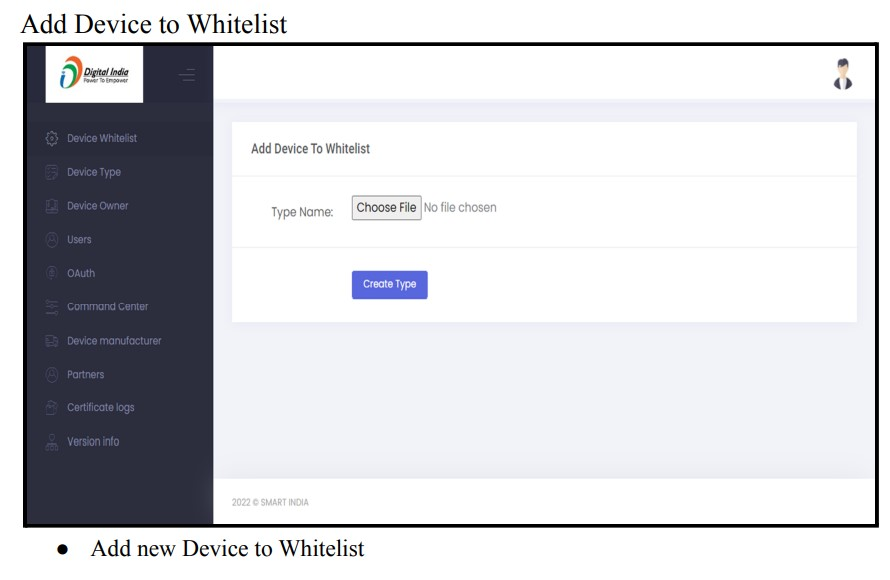
\includegraphics[height=9cm,width=14cm]{Admin/Addwhitelist.jpg}
\end{center}
\pagebreak


\begin{center}
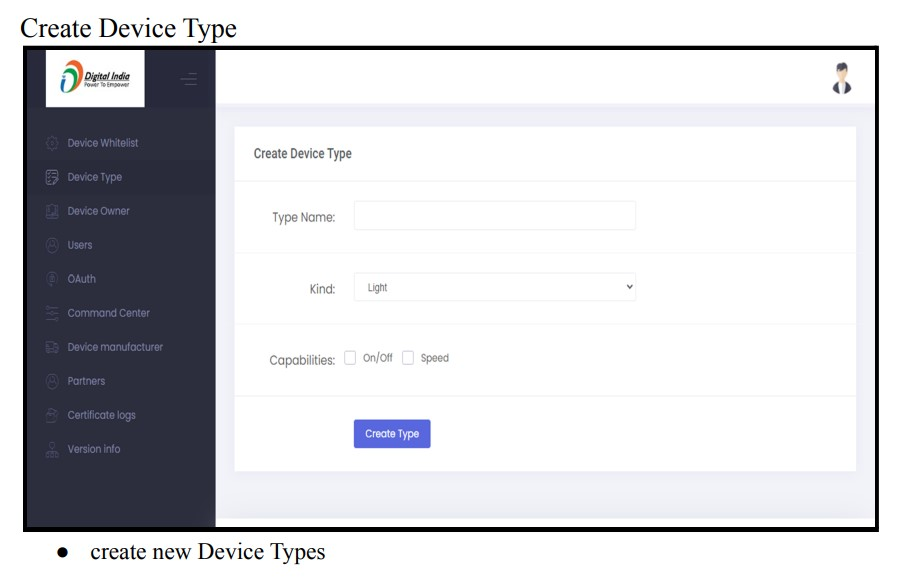
\includegraphics[height=9cm,width=14cm]{Admin/Adddivice.jpg}
\end{center}



% This section type your project contents 

\begin{center}
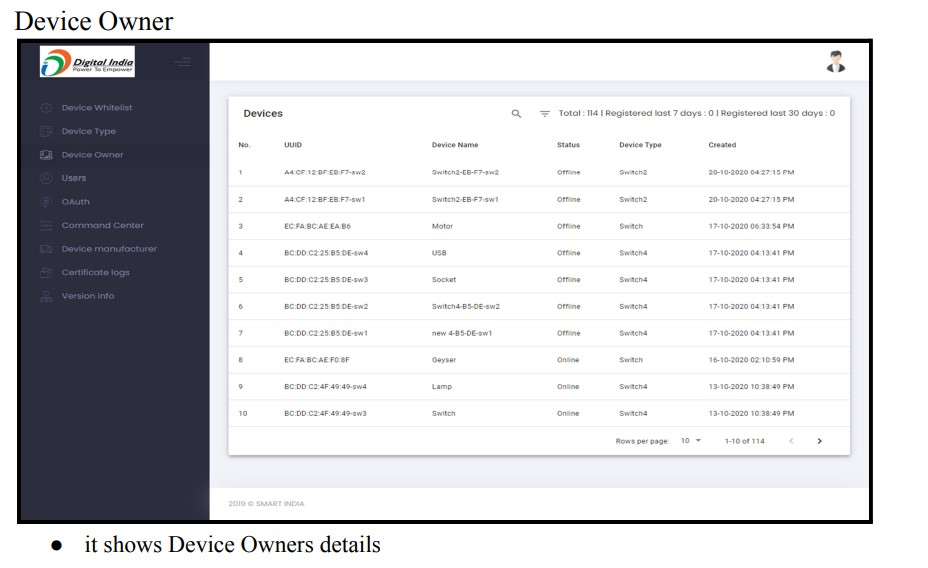
\includegraphics[height=9cm,width=14cm]{Admin/Deviceowner.jpg}
\end{center}
\pagebreak

\begin{center}
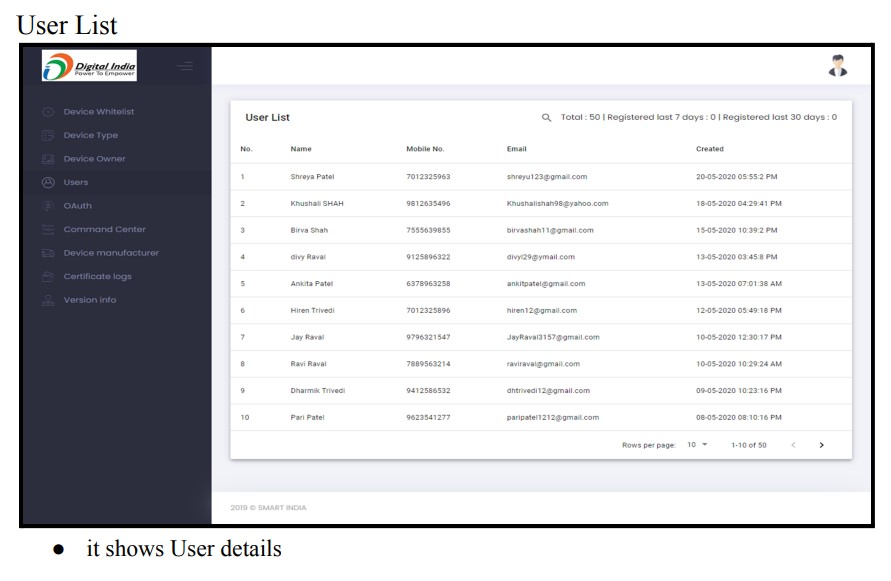
\includegraphics[height=9cm,width=14cm]{Admin/Userlist.jpg}
\end{center}

\begin{center}
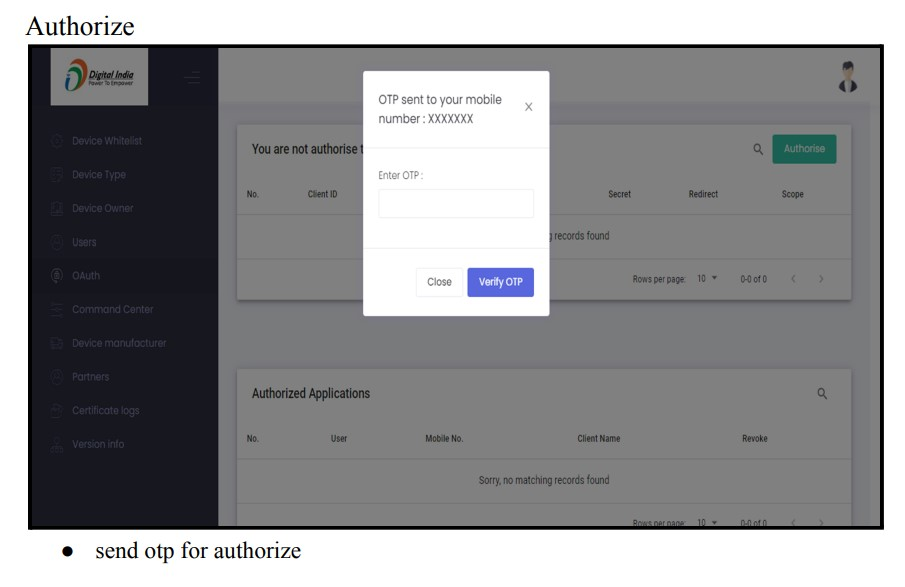
\includegraphics[height=9cm,width=14cm]{Admin/Authorize.jpg}
\end{center}
\pagebreak

\begin{center}
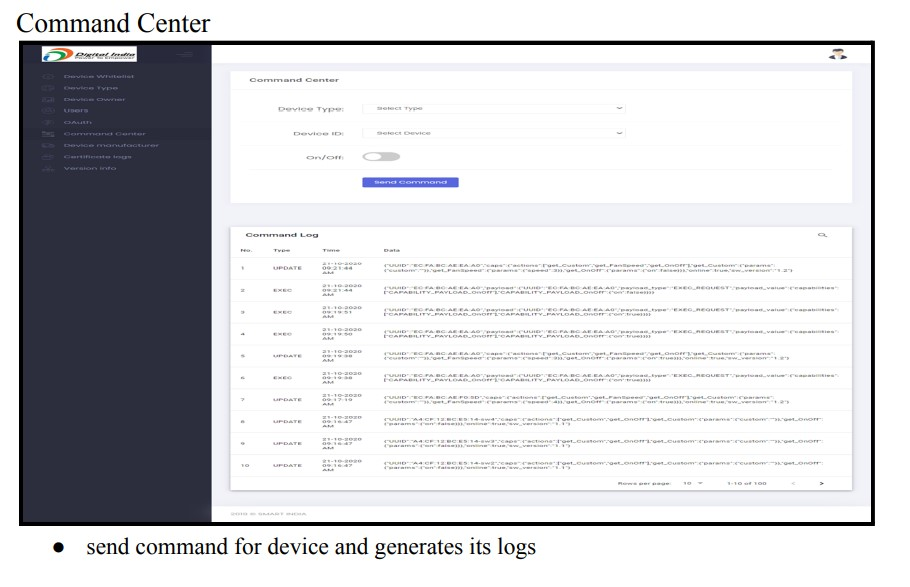
\includegraphics[height=9cm,width=14cm]{Admin/Commandcenter.jpg}
\end{center}

\begin{center}
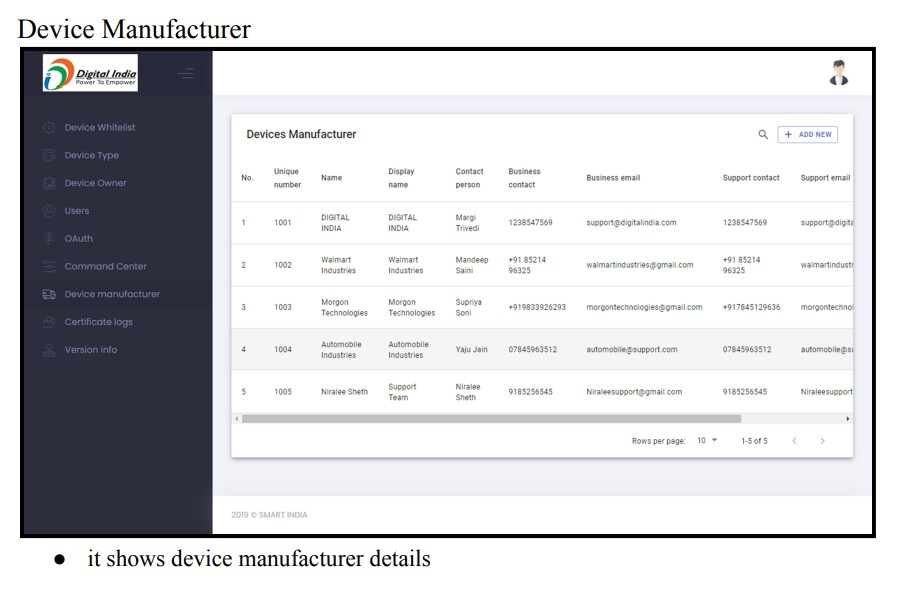
\includegraphics[height=9cm,width=14cm]{Admin/Device.jpg}
\end{center}
\pagebreak

		
		% This section type your project contents 
		
		
		
		
		
		
		
		
		
		
		
		
		
		
		
		
		
		
		
		
		
		
		
		
		
		
		
 		

\section{Database structure}
\textbf{Account Collection:}  This table stores Information for Creating account and give access to login.\nolinebreak
\begin{table}[hp]
\centering

\begin{tabular}{|c|c|c|c|}
\hline
\textbf{Field Name}  & \textbf{Data Type}  & \textbf{size} &\textbf{Constraints}  \\
\hline
name & String & 50 & NOT NULL \\
\hline
contactName &	String &	50 & NOT NULL\\
\hline
groupName & String &	50 & NOT NULL\\
\hline
isPrimaryAdmin	& Boolean & - &	NOT NULL\\
\hline
manufacturer &	Object &	- &	-\\
\hline
deviceMacId &	String & 30 &	NOT NULL\\
\hline
deviceIpAddress & String & 30 & NOT NULL\\
\hline
deviceType	& Object &	- & - \\
\hline
firmwareId	& String &	20 & NOT NULL \\
\hline
deviceName	& String &	20 & NOT NULL \\
\hline

\end{tabular}
\caption{ Account Collection}
\end{table}
\\
\textbf{Command Collection:} This table stores Commands .\nolinebreak
\begin{table}[hp]
\centering
\begin{tabular}{|c|c|c|c|}
\hline
\textbf{Field Name}  & \textbf{Data Type}  & \textbf{size} &\textbf{Constraints}  \\
\hline
command & JSON &	20 & \\
\hline

\end{tabular}
\caption{Command Collection}
\end{table}


\textbf{DeviceAuth Collection:}  This table stores Auth details .\nolinebreak

\begin{table}[hp]
\centering
\begin{tabular}{|c|c|c|c|}
\hline
\textbf{Field Name}  & \textbf{Data Type}  & \textbf{size} &\textbf{Constraints}  \\
\hline
device\_mac & String &	30 & NOT NULL\\
\hline
manufacturer\_mac & Object &	- & -\\
\hline
is\_activated\_mac & Boolean &- & NOT NULL\\
\hline
activated\_date\_mac & Date & - & NOT NULL\\
\hline

\end{tabular}
\caption{DeviceAuth Collection}
\end{table}

\pagebreak
\textbf{DeviceManufacturer Collection} This table stores Device Manufacturer Details .\nolinebreak
\begin{table}[hp]
\centering
\begin{tabular}{|c|c|c|c|}
\hline
\textbf{Field Name}  & \textbf{Data Type}  & \textbf{size} &\textbf{Constraints}  \\
\hline
name &	String &	50 & Not NULL \\\hline
uniqueNumber &	String &	20 & Not NULL \\\hline
displayName &	String &	50 & Not NULL \\\hline
contactPersonName &	String &	50 & Not NULL \\\hline
businessContactNumber &	String &	20 & Not NULL \\\hline
businessEmail &	String &	50 & Not NULL \\\hline
supportContactNumber &	String &	20 & Not NULL \\\hline
supportEmail &	String &	50 & Not NULL \\\hline
deviceType &	Object &	- & - \\\hline



 
\end{tabular}
\caption{DeviceManufacturer Collection}
\end{table}

\textbf{DeviceCapabilitiesCollection} This table stores the Device Capabilities.\nolinebreak
\begin{table}[hp]
\centering
\begin{tabular}{|c|c|c|c|}
\hline
\textbf{Field Name}  & \textbf{Data Type}  & \textbf{size} &\textbf{Constraints}  \\
\hline
name &	String &	50 & NOT NULL \\\hline
voice\_provider &	String &	50 & NOT NULL \\\hline
default\_json &	String &	30 & NOT NULL \\\hline
codegen &	Boolean &	- & NOT NULL \\\hline


 
\end{tabular}
\caption{DeviceCapabilitiesCollection}
\end{table}

\textbf{DeviceTypeCollection} This table stores the Device Type.\nolinebreak
\begin{table}[hp]
\centering
\begin{tabular}{|c|c|c|c|}
\hline
\textbf{Field Name}  & \textbf{Data Type}  & \textbf{size} &\textbf{Constraints}  \\
\hline
name &	String &	50 & NOT NULL \\\hline
deviceDefaultName &	String &	50 & NOT NULL \\\hline
icon &	String &	50 & NOT NULL \\\hline
manufacturer &	Object &	- &- \\\hline


 
\end{tabular}
\caption{DeviceTypeCollection}
\end{table}

\pagebreak

\textbf{OAuthAccessCollection} This table stores the  yearly target.\nolinebreak
\begin{table}[hp]
\centering
\begin{tabular}{|c|c|c|c|}
\hline
\textbf{Field Name}  & \textbf{Data Type}  & \textbf{size} &\textbf{Constraints}  \\
\hline
clientId &	  Object &-	 & - \\\hline
token &	String &	200 & NOT NULL \\\hline
refresh\_token &	String &	200 & NOT NULL \\\hline
revoked &	Boolean &	- & NOT NULL \\\hline

 
\end{tabular}
\caption{OAuthAccessCollection}
\end{table}


\textbf{OAuthCodeCollection} \nolinebreak
\begin{table}[hp]
\centering
\begin{tabular}{|c|c|c|c|}
\hline
\textbf{Field Name}  & \textbf{Data Type}  & \textbf{size} &\textbf{Constraints}  \\
\hline
clientId &	Object &	- & -\\\hline
code &	String &	50 & NOT NULL \\\hline
redirectUrl &	String &	200 & NOT NULL \\\hline
userName &	String &	50 & NOT NULL \\\hline
 
\end{tabular}
\caption{OAuthCodeCollection}
\end{table}

\textbf{OAuthClientCollection} This table stores the Client Auth details.\nolinebreak
\begin{table}[hp]
\centering
\begin{tabular}{|c|c|c|c|}
\hline
\textbf{Field Name}  & \textbf{Data Type}  & \textbf{size} &\textbf{Constraints}  \\
\hline
name &	String	 & 50 & NOT NULL \\\hline
display\_name &	String	 & 50 & NOT NULL \\\hline
secret &	String	 & 50 & NOT NULL \\\hline
redirect &	Array	 & 100 & NOT NULL \\\hline
notes &	String	 & 100 & NOT NULL \\\hline
revoked &	Boolen	 & - & NOT NULL \\\hline
scope &	Boolen	 & - & NOT NULL \\\hline
access\_token &	String	 & 200 & NOT NULL \\\hline
preShared\_token &	String	 & 200 & NOT NULL \\\hline
refresh\_token &	String	 & 200 & NOT NULL \\\hline


\end{tabular}
\caption{OAuthClientCollection}
\end{table}

\pagebreak

\textbf{OtpCollection} This table stores the  details For OTP.\nolinebreak
\begin{table}[hp]
\centering
\begin{tabular}{|c|c|c|c|}
\hline
\textbf{Field Name}  & \textbf{Data Type}  & \textbf{size} &\textbf{Constraints}  \\
\hline
mobileNo & String &	20 & NOT NULL \\\hline
Otp & String &	10 & NOT NULL \\\hline
otpValidThrough & Date &	- & NOT NULL \\\hline

\end{tabular}
\caption{OtpCollection}
\end{table}

\textbf{WhitelistDevicesCollection} This table stores the user Whitelist details.\nolinebreak
\begin{table}[hp]
\centering
\begin{tabular}{|c|c|c|c|}
\hline
\textbf{Field Name}  & \textbf{Data Type}  & \textbf{size} &\textbf{Constraints}  \\
\hline
UUID & String &	50 & NOT NULL \\\hline
manufacturer & Object &	- & - \\\hline
isActivat & Boolen &	- & NOT NULL \\\hline

\end{tabular}
\caption{WhitelistDevicesCollection}
\end{table}



\textbf{VersionInfoCollection} This table stores the Device Version details.\nolinebreak
\begin{table}[hp]
\centering
\begin{tabular}{|c|c|c|c|}
\hline
\textbf{Field Name}  & \textbf{Data Type}  & \textbf{size} &\textbf{Constraints}  \\
\hline
deviceVersion & String &	50 & NOT NULL \\\hline
deviceType & Object &	- & - \\\hline
apiVersion & String &	50 & NOT NULL \\\hline
deviceUniqueId & String &	50 & NOT NULL \\\hline
  

\end{tabular}
\caption{VersionInfoCollection}
\end{table}



